\section{Theorie}
 \label{sec:Theorie}
Werden Metalloberflächen mit Licht bestrahlt so treten Elektronen aus dieser aus.
Diese Beobachtung nennt sich Photoeffekt. Wird der Metalloberfläche, welche auch Photokathode genannt wird,
eine zweite Metallplatte, mit positivem Potential, gegenüber gestellt, so kann mit einem Strommessgerät ein
Strom gemessen werden. Der prinzipielle Aufbau findet sich in Abbildung \ref{fig:aufbau}.
\begin{figure}
  \centering
 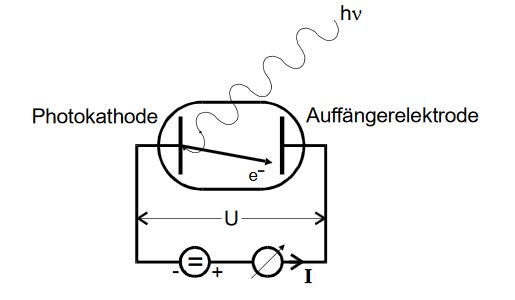
\includegraphics[width=0.7\textwidth]{aufbau.png}
\caption{Exemplarischer Aufbau zur Untersuchung des Photoeffekts.\cite{sample}}
 \label{fig:aufbau}
  \end{figure}
  Im Experiment werden folgende Zusammenhänge erschlossen:
  \begin{itemize}
    \item Die pro Zeiteinheit austretenden Elektronen sind proportional zur Lichtintensität.
    \item Die Energie der Elektronen ist abhängig von der Lichtfrequenz $\nu$ und nicht von der Intensität.
    \item Der Photoeffekt trrit erst ab einer Grundfrequenz auf.
  \end{itemize}
  Mit der Wellentheorie des Lichts können diese Erscheinungen nicht erklärt werden.
  Hierbei wird angenommen, dass die Elektronen durch die einfallenden elektromagnetischen Wellen zum Schwingen angeregt werden.
  Durch die Energieübertragung wird die Schwingungsamplitude immer größer, bis Elektronen in der Lage sind auszutreten.
  Damit wäre die Energie der Elektronen aber von der Intensität des Lichts abhängig.
  Mit einem Teilchenmodell des Lichts können die Beobachtungen erklärt werden.
  Die Photonen breiten sich mit Lichtgeschwindigkeit aus und besitzen alle die Energie $E=\mathrm{h}\nu$, $\mathrm{h}$ ist das planksche
  Wirkungsquantum. Ein Photon gibt seine gesamte Energie an ein Elektron ab, diese Teilt sich in die Austrittsarbeit $A_\mathrm{k}$ und
  die kinetische Energie auf:
  \begin{align*}
  \mathrm{h}\nu=E_\mathrm{kin} + A_\mathrm{k}.\\
  \end{align*}
  Mit $\mathrm{h}\nu < A_\mathrm{k}$ lässt sich die Grenzfrequenz erklären.
  Die Abhängigkeit von der Intensität ist ebenfalls mit dem Teilchencharakter vereinbar, je mehr Teilchen auf die Oberfläche treffen,
  desto mehr Elektronen werden ausgelöst.
